\section{src/physics/test\_\-ode.cpp File Reference}
\label{test__ode_8cpp}\index{src/physics/test_ode.cpp@{src/physics/test\_\-ode.cpp}}
{\tt \#include $<$setjmp.h$>$}\par
{\tt \#include $<$ode/ode.h$>$}\par


Include dependency graph for test\_\-ode.cpp:\begin{figure}[H]
\begin{center}
\leavevmode
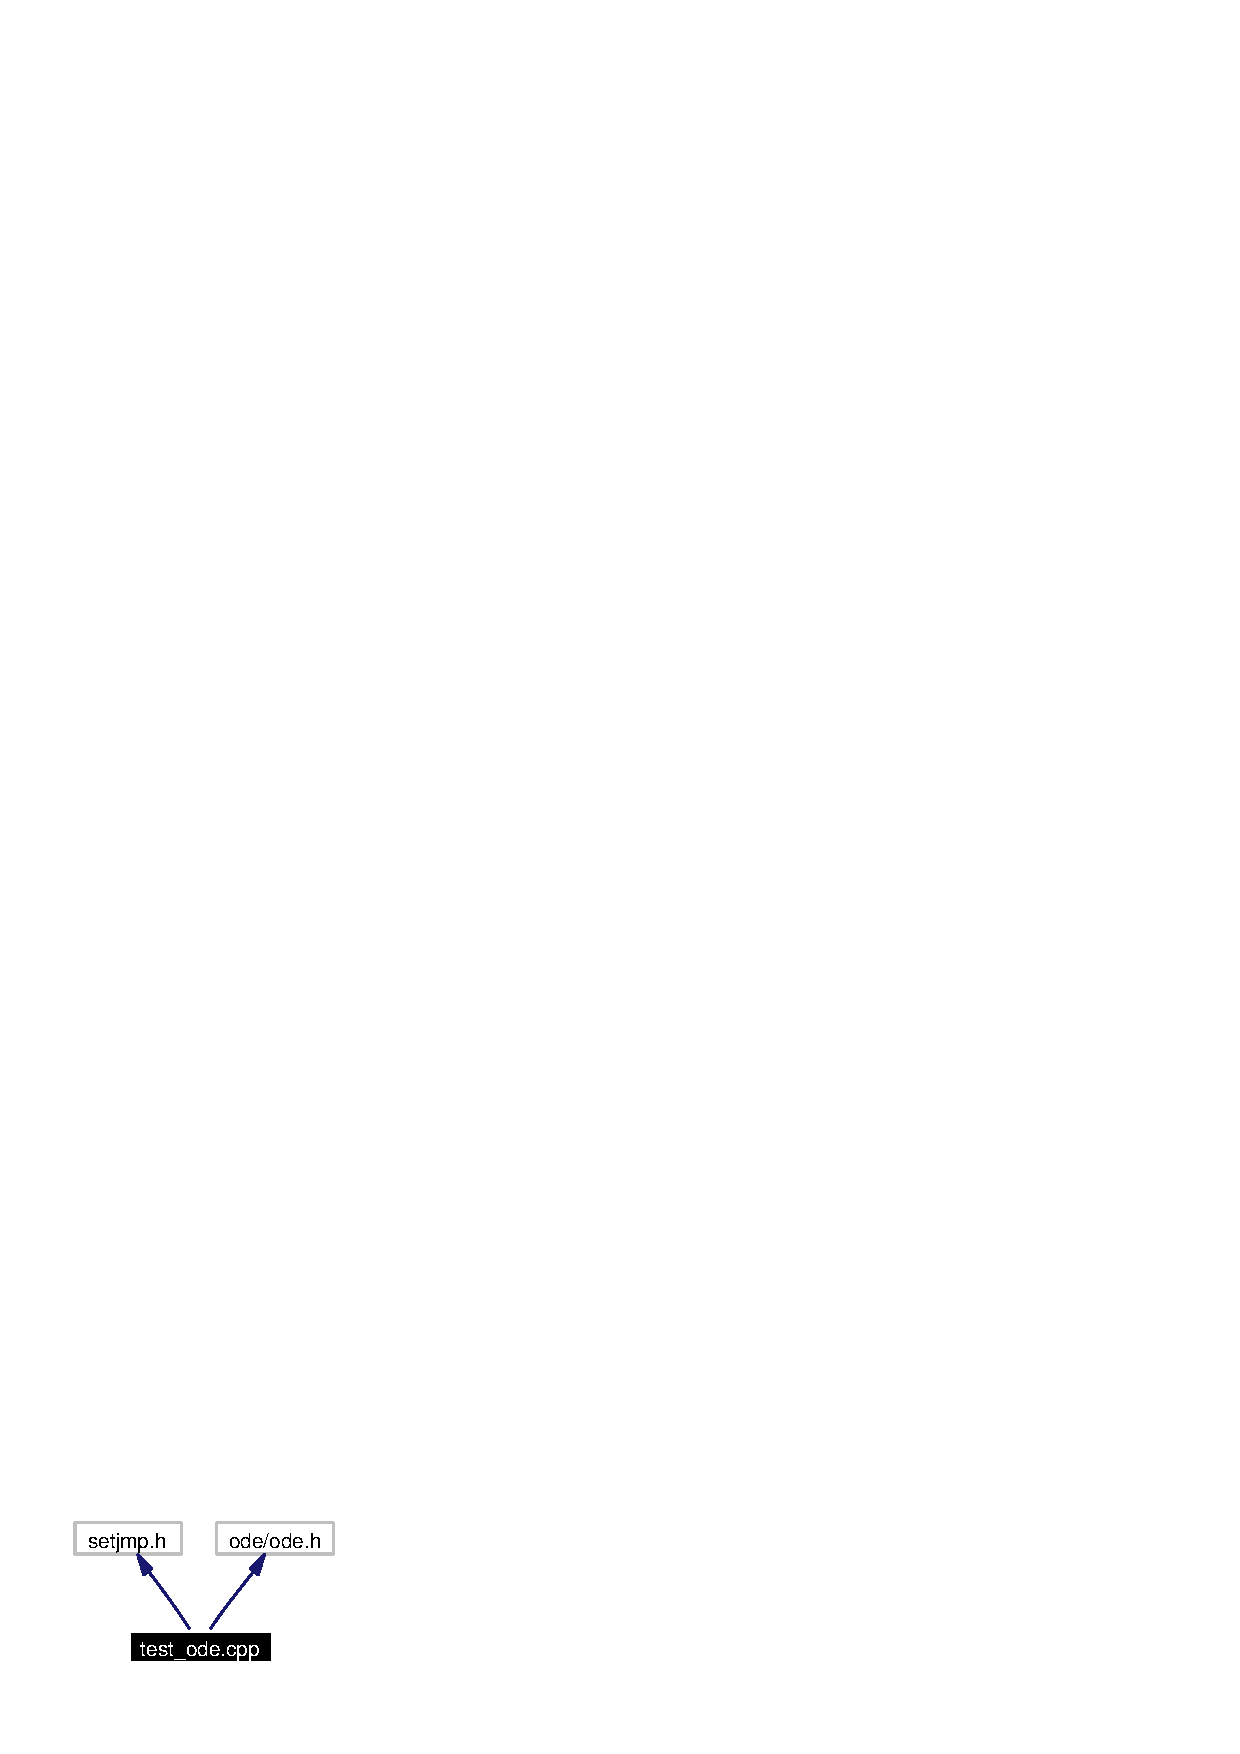
\includegraphics[width=80pt]{test__ode_8cpp__incl}
\end{center}
\end{figure}


This graph shows which files directly or indirectly include this file:\begin{figure}[H]
\begin{center}
\leavevmode
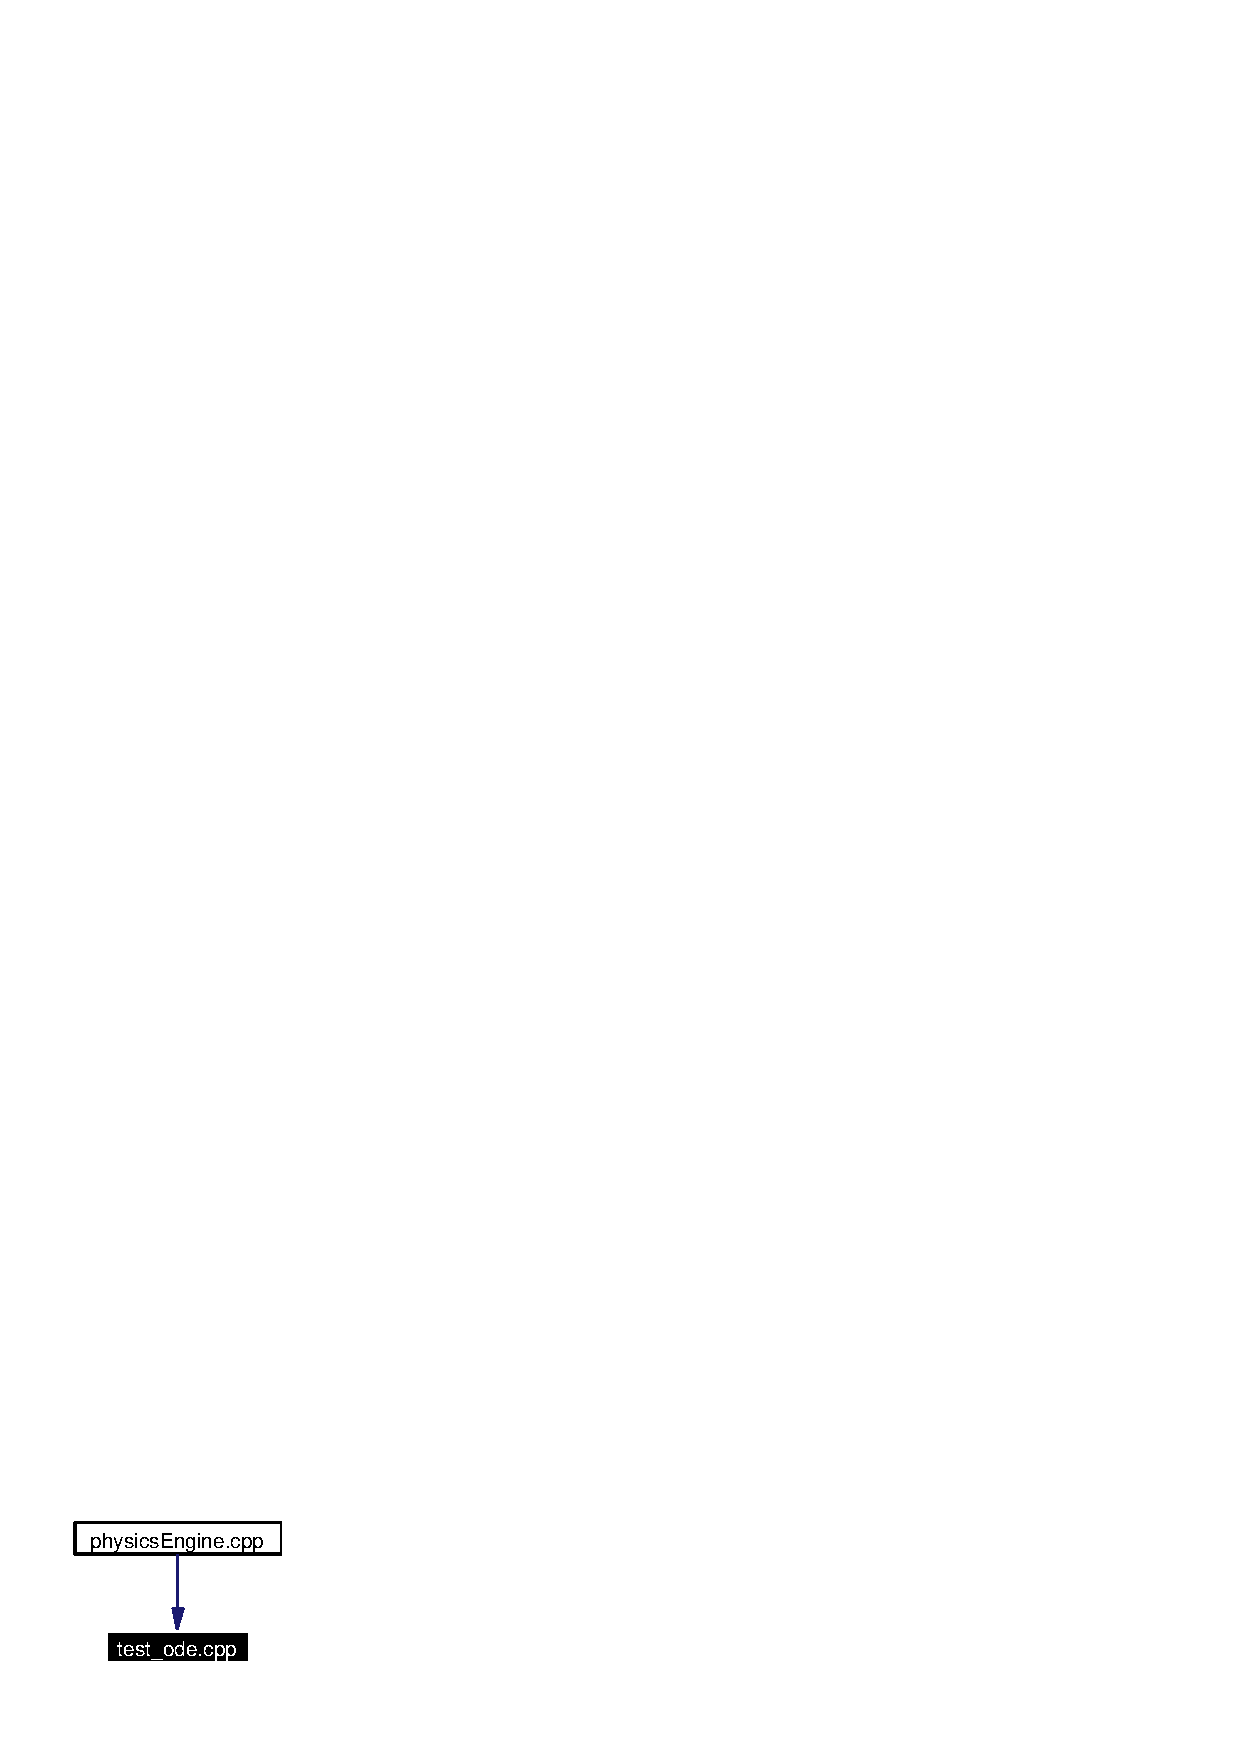
\includegraphics[width=67pt]{test__ode_8cpp__dep__incl}
\end{center}
\end{figure}
\subsection*{Defines}
\begin{CompactItemize}
\item 
\#define {\bf \_\-A}(i, j)\ A[(i)$\ast$4+(j)]
\item 
\#define {\bf \_\-I}(i, j)\ I[(i)$\ast$4+(j)]
\item 
\#define {\bf \_\-R}(i, j)\ R[(i)$\ast$4+(j)]
\item 
\#define {\bf HEADER}\ printf (\char`\"{}\%s:\%d$\backslash$n\char`\"{},\_\-\_\-FILE\_\-\_\-,\_\-\_\-LINE\_\-\_\-);
\item 
\#define {\bf TRAP\_\-MESSAGE}(do, ifnomsg, ifmsg)
\item 
\#define {\bf MSIZE}\ 21
\item 
\#define {\bf MSIZE4}\ 24
\item 
\#define {\bf NUMP}\ 10
\end{CompactItemize}
\subsection*{Functions}
\begin{CompactItemize}
\item 
void {\bf my\-Message\-Function} (int num, const char $\ast$msg, va\_\-list ap)
\item 
int {\bf cmp} (d\-Real a, d\-Real b)
\item 
int {\bf cmp\-Identity\-Mat3} (d\-Matrix3 A)
\item 
void {\bf transpose3x3} (d\-Matrix3 A)
\item 
void {\bf test\-Random\-Number\-Generator} ()
\item 
void {\bf test\-Infinity} ()
\item 
void {\bf test\-Pad} ()
\item 
void {\bf test\-Cross\-Product} ()
\item 
void {\bf test\-Set\-Zero} ()
\item 
void {\bf test\-Normalize3} ()
\item 
void {\bf test\-Plane\-Space} ()
\item 
void {\bf test\-Matrix\-Multiply} ()
\item 
void {\bf test\-Small\-Matrix\-Multiply} ()
\item 
void {\bf test\-Cholesky\-Factorization} ()
\item 
void {\bf test\-Cholesky\-Solve} ()
\item 
void {\bf test\-Invert\-PDMatrix} ()
\item 
void {\bf test\-Is\-Positive\-Definite} ()
\item 
void {\bf test\-Fast\-LDLTFactorization} ()
\item 
void {\bf test\-Solve\-LDLT} ()
\item 
void {\bf test\-LDLTAdd\-TL} ()
\item 
void {\bf test\-LDLTRemove} ()
\item 
void {\bf print\-Mass\-Params} (d\-Mass $\ast$m)
\item 
void {\bf compare\-Mass\-Params} (d\-Mass $\ast$m1, d\-Mass $\ast$m2, char $\ast$msg)
\item 
void {\bf compute\-Mass\-Params} (d\-Mass $\ast$m, d\-Real q[NUMP][3], d\-Real pm[NUMP])
\item 
void {\bf test\-Mass\-Functions} ()
\item 
void {\bf make\-Random\-Rotation} (d\-Matrix3 R)
\item 
void {\bf test\-Rto\-Qand\-Qto\-R} ()
\item 
void {\bf test\-Quaternion\-Multiply} ()
\item 
void {\bf test\-Rotation\-Functions} ()
\item 
void {\bf d\-Test\-Data\-Structures} ()
\item 
void {\bf d\-Test\-Matrix\-Comparison} ()
\item 
void {\bf d\-Test\-Solve\-LCP} ()
\item 
int {\bf test\-Ode} (void)
\item 
void {\bf test\-Ode2} (void)
\end{CompactItemize}
\subsection*{Variables}
\begin{CompactItemize}
\item 
jmp\_\-buf {\bf jump\_\-buffer}
\end{CompactItemize}


\subsection{Define Documentation}
\index{test_ode.cpp@{test\_\-ode.cpp}!_A@{\_\-A}}
\index{_A@{\_\-A}!test_ode.cpp@{test\_\-ode.cpp}}
\subsubsection{\setlength{\rightskip}{0pt plus 5cm}\#define \_\-A(i, j)\ A[(i)$\ast$4+(j)]}\label{test__ode_8cpp_a0}


\index{test_ode.cpp@{test\_\-ode.cpp}!_I@{\_\-I}}
\index{_I@{\_\-I}!test_ode.cpp@{test\_\-ode.cpp}}
\subsubsection{\setlength{\rightskip}{0pt plus 5cm}\#define \_\-I(i, j)\ I[(i)$\ast$4+(j)]}\label{test__ode_8cpp_a1}


\index{test_ode.cpp@{test\_\-ode.cpp}!_R@{\_\-R}}
\index{_R@{\_\-R}!test_ode.cpp@{test\_\-ode.cpp}}
\subsubsection{\setlength{\rightskip}{0pt plus 5cm}\#define \_\-R(i, j)\ R[(i)$\ast$4+(j)]}\label{test__ode_8cpp_a2}


\index{test_ode.cpp@{test\_\-ode.cpp}!HEADER@{HEADER}}
\index{HEADER@{HEADER}!test_ode.cpp@{test\_\-ode.cpp}}
\subsubsection{\setlength{\rightskip}{0pt plus 5cm}\#define HEADER\ printf (\char`\"{}\%s:\%d$\backslash$n\char`\"{},\_\-\_\-FILE\_\-\_\-,\_\-\_\-LINE\_\-\_\-);}\label{test__ode_8cpp_a3}


\index{test_ode.cpp@{test\_\-ode.cpp}!MSIZE@{MSIZE}}
\index{MSIZE@{MSIZE}!test_ode.cpp@{test\_\-ode.cpp}}
\subsubsection{\setlength{\rightskip}{0pt plus 5cm}\#define MSIZE\ 21}\label{test__ode_8cpp_a5}


\index{test_ode.cpp@{test\_\-ode.cpp}!MSIZE4@{MSIZE4}}
\index{MSIZE4@{MSIZE4}!test_ode.cpp@{test\_\-ode.cpp}}
\subsubsection{\setlength{\rightskip}{0pt plus 5cm}\#define MSIZE4\ 24}\label{test__ode_8cpp_a6}


\index{test_ode.cpp@{test\_\-ode.cpp}!NUMP@{NUMP}}
\index{NUMP@{NUMP}!test_ode.cpp@{test\_\-ode.cpp}}
\subsubsection{\setlength{\rightskip}{0pt plus 5cm}\#define NUMP\ 10}\label{test__ode_8cpp_a7}


\index{test_ode.cpp@{test\_\-ode.cpp}!TRAP_MESSAGE@{TRAP\_\-MESSAGE}}
\index{TRAP_MESSAGE@{TRAP\_\-MESSAGE}!test_ode.cpp@{test\_\-ode.cpp}}
\subsubsection{\setlength{\rightskip}{0pt plus 5cm}\#define TRAP\_\-MESSAGE(do, ifnomsg, ifmsg)}\label{test__ode_8cpp_a4}


{\bf Value:}

\footnotesize\begin{verbatim}dSetMessageHandler (&myMessageFunction); \
  if (setjmp (jump_buffer)) { \
    dSetMessageHandler (0); \
    ifmsg ; \
  } \
  else { \
    dSetMessageHandler (&myMessageFunction); \
    do ; \
    ifnomsg ; \
  } \
  dSetMessageHandler (0);
\end{verbatim}\normalsize 


\subsection{Function Documentation}
\index{test_ode.cpp@{test\_\-ode.cpp}!cmp@{cmp}}
\index{cmp@{cmp}!test_ode.cpp@{test\_\-ode.cpp}}
\subsubsection{\setlength{\rightskip}{0pt plus 5cm}int cmp (d\-Real {\em a}, d\-Real {\em b})}\label{test__ode_8cpp_a10}


\index{test_ode.cpp@{test\_\-ode.cpp}!cmpIdentityMat3@{cmpIdentityMat3}}
\index{cmpIdentityMat3@{cmpIdentityMat3}!test_ode.cpp@{test\_\-ode.cpp}}
\subsubsection{\setlength{\rightskip}{0pt plus 5cm}int cmp\-Identity\-Mat3 (d\-Matrix3 {\em A})}\label{test__ode_8cpp_a11}


\index{test_ode.cpp@{test\_\-ode.cpp}!compareMassParams@{compareMassParams}}
\index{compareMassParams@{compareMassParams}!test_ode.cpp@{test\_\-ode.cpp}}
\subsubsection{\setlength{\rightskip}{0pt plus 5cm}void compare\-Mass\-Params (d\-Mass $\ast$ {\em m1}, d\-Mass $\ast$ {\em m2}, char $\ast$ {\em msg})}\label{test__ode_8cpp_a31}


\index{test_ode.cpp@{test\_\-ode.cpp}!computeMassParams@{computeMassParams}}
\index{computeMassParams@{computeMassParams}!test_ode.cpp@{test\_\-ode.cpp}}
\subsubsection{\setlength{\rightskip}{0pt plus 5cm}void compute\-Mass\-Params (d\-Mass $\ast$ {\em m}, d\-Real {\em q}[NUMP][3], d\-Real {\em pm}[NUMP])}\label{test__ode_8cpp_a32}


\index{test_ode.cpp@{test\_\-ode.cpp}!dTestDataStructures@{dTestDataStructures}}
\index{dTestDataStructures@{dTestDataStructures}!test_ode.cpp@{test\_\-ode.cpp}}
\subsubsection{\setlength{\rightskip}{0pt plus 5cm}void d\-Test\-Data\-Structures ()}\label{test__ode_8cpp_a38}


\index{test_ode.cpp@{test\_\-ode.cpp}!dTestMatrixComparison@{dTestMatrixComparison}}
\index{dTestMatrixComparison@{dTestMatrixComparison}!test_ode.cpp@{test\_\-ode.cpp}}
\subsubsection{\setlength{\rightskip}{0pt plus 5cm}void d\-Test\-Matrix\-Comparison ()}\label{test__ode_8cpp_a39}


\index{test_ode.cpp@{test\_\-ode.cpp}!dTestSolveLCP@{dTestSolveLCP}}
\index{dTestSolveLCP@{dTestSolveLCP}!test_ode.cpp@{test\_\-ode.cpp}}
\subsubsection{\setlength{\rightskip}{0pt plus 5cm}void d\-Test\-Solve\-LCP ()}\label{test__ode_8cpp_a40}


\index{test_ode.cpp@{test\_\-ode.cpp}!makeRandomRotation@{makeRandomRotation}}
\index{makeRandomRotation@{makeRandomRotation}!test_ode.cpp@{test\_\-ode.cpp}}
\subsubsection{\setlength{\rightskip}{0pt plus 5cm}void make\-Random\-Rotation (d\-Matrix3 {\em R})}\label{test__ode_8cpp_a34}


\index{test_ode.cpp@{test\_\-ode.cpp}!myMessageFunction@{myMessageFunction}}
\index{myMessageFunction@{myMessageFunction}!test_ode.cpp@{test\_\-ode.cpp}}
\subsubsection{\setlength{\rightskip}{0pt plus 5cm}void my\-Message\-Function (int {\em num}, const char $\ast$ {\em msg}, va\_\-list {\em ap})}\label{test__ode_8cpp_a9}


\index{test_ode.cpp@{test\_\-ode.cpp}!printMassParams@{printMassParams}}
\index{printMassParams@{printMassParams}!test_ode.cpp@{test\_\-ode.cpp}}
\subsubsection{\setlength{\rightskip}{0pt plus 5cm}void print\-Mass\-Params (d\-Mass $\ast$ {\em m})}\label{test__ode_8cpp_a30}


\index{test_ode.cpp@{test\_\-ode.cpp}!testCholeskyFactorization@{testCholeskyFactorization}}
\index{testCholeskyFactorization@{testCholeskyFactorization}!test_ode.cpp@{test\_\-ode.cpp}}
\subsubsection{\setlength{\rightskip}{0pt plus 5cm}void test\-Cholesky\-Factorization ()}\label{test__ode_8cpp_a22}


\index{test_ode.cpp@{test\_\-ode.cpp}!testCholeskySolve@{testCholeskySolve}}
\index{testCholeskySolve@{testCholeskySolve}!test_ode.cpp@{test\_\-ode.cpp}}
\subsubsection{\setlength{\rightskip}{0pt plus 5cm}void test\-Cholesky\-Solve ()}\label{test__ode_8cpp_a23}


\index{test_ode.cpp@{test\_\-ode.cpp}!testCrossProduct@{testCrossProduct}}
\index{testCrossProduct@{testCrossProduct}!test_ode.cpp@{test\_\-ode.cpp}}
\subsubsection{\setlength{\rightskip}{0pt plus 5cm}void test\-Cross\-Product ()}\label{test__ode_8cpp_a16}


\index{test_ode.cpp@{test\_\-ode.cpp}!testFastLDLTFactorization@{testFastLDLTFactorization}}
\index{testFastLDLTFactorization@{testFastLDLTFactorization}!test_ode.cpp@{test\_\-ode.cpp}}
\subsubsection{\setlength{\rightskip}{0pt plus 5cm}void test\-Fast\-LDLTFactorization ()}\label{test__ode_8cpp_a26}


\index{test_ode.cpp@{test\_\-ode.cpp}!testInfinity@{testInfinity}}
\index{testInfinity@{testInfinity}!test_ode.cpp@{test\_\-ode.cpp}}
\subsubsection{\setlength{\rightskip}{0pt plus 5cm}void test\-Infinity ()}\label{test__ode_8cpp_a14}


\index{test_ode.cpp@{test\_\-ode.cpp}!testInvertPDMatrix@{testInvertPDMatrix}}
\index{testInvertPDMatrix@{testInvertPDMatrix}!test_ode.cpp@{test\_\-ode.cpp}}
\subsubsection{\setlength{\rightskip}{0pt plus 5cm}void test\-Invert\-PDMatrix ()}\label{test__ode_8cpp_a24}


\index{test_ode.cpp@{test\_\-ode.cpp}!testIsPositiveDefinite@{testIsPositiveDefinite}}
\index{testIsPositiveDefinite@{testIsPositiveDefinite}!test_ode.cpp@{test\_\-ode.cpp}}
\subsubsection{\setlength{\rightskip}{0pt plus 5cm}void test\-Is\-Positive\-Definite ()}\label{test__ode_8cpp_a25}


\index{test_ode.cpp@{test\_\-ode.cpp}!testLDLTAddTL@{testLDLTAddTL}}
\index{testLDLTAddTL@{testLDLTAddTL}!test_ode.cpp@{test\_\-ode.cpp}}
\subsubsection{\setlength{\rightskip}{0pt plus 5cm}void test\-LDLTAdd\-TL ()}\label{test__ode_8cpp_a28}


\index{test_ode.cpp@{test\_\-ode.cpp}!testLDLTRemove@{testLDLTRemove}}
\index{testLDLTRemove@{testLDLTRemove}!test_ode.cpp@{test\_\-ode.cpp}}
\subsubsection{\setlength{\rightskip}{0pt plus 5cm}void test\-LDLTRemove ()}\label{test__ode_8cpp_a29}


\index{test_ode.cpp@{test\_\-ode.cpp}!testMassFunctions@{testMassFunctions}}
\index{testMassFunctions@{testMassFunctions}!test_ode.cpp@{test\_\-ode.cpp}}
\subsubsection{\setlength{\rightskip}{0pt plus 5cm}void test\-Mass\-Functions ()}\label{test__ode_8cpp_a33}


\index{test_ode.cpp@{test\_\-ode.cpp}!testMatrixMultiply@{testMatrixMultiply}}
\index{testMatrixMultiply@{testMatrixMultiply}!test_ode.cpp@{test\_\-ode.cpp}}
\subsubsection{\setlength{\rightskip}{0pt plus 5cm}void test\-Matrix\-Multiply ()}\label{test__ode_8cpp_a20}


\index{test_ode.cpp@{test\_\-ode.cpp}!testNormalize3@{testNormalize3}}
\index{testNormalize3@{testNormalize3}!test_ode.cpp@{test\_\-ode.cpp}}
\subsubsection{\setlength{\rightskip}{0pt plus 5cm}void test\-Normalize3 ()}\label{test__ode_8cpp_a18}


\index{test_ode.cpp@{test\_\-ode.cpp}!testOde@{testOde}}
\index{testOde@{testOde}!test_ode.cpp@{test\_\-ode.cpp}}
\subsubsection{\setlength{\rightskip}{0pt plus 5cm}int test\-Ode (void)}\label{test__ode_8cpp_a41}


\index{test_ode.cpp@{test\_\-ode.cpp}!testOde2@{testOde2}}
\index{testOde2@{testOde2}!test_ode.cpp@{test\_\-ode.cpp}}
\subsubsection{\setlength{\rightskip}{0pt plus 5cm}void test\-Ode2 (void)}\label{test__ode_8cpp_a42}


\index{test_ode.cpp@{test\_\-ode.cpp}!testPad@{testPad}}
\index{testPad@{testPad}!test_ode.cpp@{test\_\-ode.cpp}}
\subsubsection{\setlength{\rightskip}{0pt plus 5cm}void test\-Pad ()}\label{test__ode_8cpp_a15}


\index{test_ode.cpp@{test\_\-ode.cpp}!testPlaneSpace@{testPlaneSpace}}
\index{testPlaneSpace@{testPlaneSpace}!test_ode.cpp@{test\_\-ode.cpp}}
\subsubsection{\setlength{\rightskip}{0pt plus 5cm}void test\-Plane\-Space ()}\label{test__ode_8cpp_a19}


\index{test_ode.cpp@{test\_\-ode.cpp}!testQuaternionMultiply@{testQuaternionMultiply}}
\index{testQuaternionMultiply@{testQuaternionMultiply}!test_ode.cpp@{test\_\-ode.cpp}}
\subsubsection{\setlength{\rightskip}{0pt plus 5cm}void test\-Quaternion\-Multiply ()}\label{test__ode_8cpp_a36}


\index{test_ode.cpp@{test\_\-ode.cpp}!testRandomNumberGenerator@{testRandomNumberGenerator}}
\index{testRandomNumberGenerator@{testRandomNumberGenerator}!test_ode.cpp@{test\_\-ode.cpp}}
\subsubsection{\setlength{\rightskip}{0pt plus 5cm}void test\-Random\-Number\-Generator ()}\label{test__ode_8cpp_a13}


\index{test_ode.cpp@{test\_\-ode.cpp}!testRotationFunctions@{testRotationFunctions}}
\index{testRotationFunctions@{testRotationFunctions}!test_ode.cpp@{test\_\-ode.cpp}}
\subsubsection{\setlength{\rightskip}{0pt plus 5cm}void test\-Rotation\-Functions ()}\label{test__ode_8cpp_a37}


\index{test_ode.cpp@{test\_\-ode.cpp}!testRtoQandQtoR@{testRtoQandQtoR}}
\index{testRtoQandQtoR@{testRtoQandQtoR}!test_ode.cpp@{test\_\-ode.cpp}}
\subsubsection{\setlength{\rightskip}{0pt plus 5cm}void test\-Rto\-Qand\-Qto\-R ()}\label{test__ode_8cpp_a35}


\index{test_ode.cpp@{test\_\-ode.cpp}!testSetZero@{testSetZero}}
\index{testSetZero@{testSetZero}!test_ode.cpp@{test\_\-ode.cpp}}
\subsubsection{\setlength{\rightskip}{0pt plus 5cm}void test\-Set\-Zero ()}\label{test__ode_8cpp_a17}


\index{test_ode.cpp@{test\_\-ode.cpp}!testSmallMatrixMultiply@{testSmallMatrixMultiply}}
\index{testSmallMatrixMultiply@{testSmallMatrixMultiply}!test_ode.cpp@{test\_\-ode.cpp}}
\subsubsection{\setlength{\rightskip}{0pt plus 5cm}void test\-Small\-Matrix\-Multiply ()}\label{test__ode_8cpp_a21}


\index{test_ode.cpp@{test\_\-ode.cpp}!testSolveLDLT@{testSolveLDLT}}
\index{testSolveLDLT@{testSolveLDLT}!test_ode.cpp@{test\_\-ode.cpp}}
\subsubsection{\setlength{\rightskip}{0pt plus 5cm}void test\-Solve\-LDLT ()}\label{test__ode_8cpp_a27}


\index{test_ode.cpp@{test\_\-ode.cpp}!transpose3x3@{transpose3x3}}
\index{transpose3x3@{transpose3x3}!test_ode.cpp@{test\_\-ode.cpp}}
\subsubsection{\setlength{\rightskip}{0pt plus 5cm}void transpose3x3 (d\-Matrix3 {\em A})}\label{test__ode_8cpp_a12}




\subsection{Variable Documentation}
\index{test_ode.cpp@{test\_\-ode.cpp}!jump_buffer@{jump\_\-buffer}}
\index{jump_buffer@{jump\_\-buffer}!test_ode.cpp@{test\_\-ode.cpp}}
\subsubsection{\setlength{\rightskip}{0pt plus 5cm}jmp\_\-buf {\bf jump\_\-buffer}\hspace{0.3cm}{\tt  [static]}}\label{test__ode_8cpp_a8}


